\documentclass{article}
\usepackage[spanish]{babel}
\usepackage[numbers,sort&compress]{natbib}
\usepackage{graphicx}
\usepackage{url}
\usepackage{amsmath}
\usepackage{hyperref}
\usepackage{float}
\usepackage{color}
\definecolor{gray86}{gray}{.86}
\definecolor{gray75}{gray}{.75}
\definecolor{gray45}{gray}{.45}
\usepackage{listings}
\lstset{ 
language=C,                
basicstyle=\footnotesize,      
numbers=left,                  
numberstyle=\footnotesize,     
stepnumber=1,                   
numbersep=5pt,                  
backgroundcolor=\color{gray86},  
showspaces=false,              
showstringspaces=false,         
showtabs=false,                
frame=single,           
tabsize=2,          
captionpos=b,          
breaklines=true,        
breakatwhitespace=false,   
escapeinside={\%*}{*)}          
}
\usepackage{subfigure} 
\usepackage[top=15mm, bottom=15mm, left=15mm, right=15mm]{geometry}
\setlength{\parskip}{2mm}
\setlength{\parindent}{0pt}

\author{Abraham Azael Morales Juárez  1422745}
\title{Búsqueda Local}
\date{\today}

\begin{document}

\maketitle

\section{Introducción}
Se generarán funciones capaces de detectar máximos locales. Primeramente, se realizará una función en una dimensión, donde se minimiza la función f(x). Será necesario realizar una función bidimencional g(x, y). Está nueva función debe poder identificar los máximos locales. Es posible implementar métodos eficientes \cite{REF1} para identificar los valores determinados por las máximas locales de una función\cite{REF2}. 

\section{Objetivos}
Realizar combinaciones que proporcionan ocho posiciones posibles vecinos.\\
Graficar en tres dimensiones.\\
Crear una visualización animada de cómo proceden 15 réplicas simultáneas de la búsqueda encima de una gráfica de proyección plana.

\section{Resultados}
Se modificó el código final que fue proporcionado (1) para agregar la función g(x,y).
\begin{lstlisting}[frame=single]
g <- function(x, y) {
  return(((x + 0.5)^4 - 30 * x^2 - 20 * x + (y + 0.5)^4 - 30 * y^2 - 20 * y)/100)
}
  \end{lstlisting}
  
Además se modificó el código para la generación de vecinos, donde se colocó la opción para poder generar 8 distintas posiciones que pudiese elegir para posicionarse. Se coloca el fragmento del código a continuación.

\begin{lstlisting}[frame=single]
replica <- function(t) {
  curr <- runif(2, low, high)
  best <- curr
  for (tiempo in 1:t) {
    deltax <- runif(1,0,step)
    deltay <- runif(1,0,step)
    
    up <- best + deltay
    down <- best - deltay
    right <- best + deltax
    left <- best - deltax
    
    upright <- best + c(deltax,deltay)
    upleft <- best + c(-deltax,deltay)
    
    downright <- best + c(deltax,-deltay)
    downleft <- best +c(-deltax,-deltay)
   
    \end{lstlisting}

Los resultados obtenidos se pueden observar en la Figura 1 y 2, donde una línea verde representa el valor máximo real del experimento, y se puede observar como la línea va cambiando según los pasos que se estén dando. Hubo un inconveniente, no se pudo hacer que el código marcara los puntos del análisis en rojo.
\begin{figure}[H]
\centering
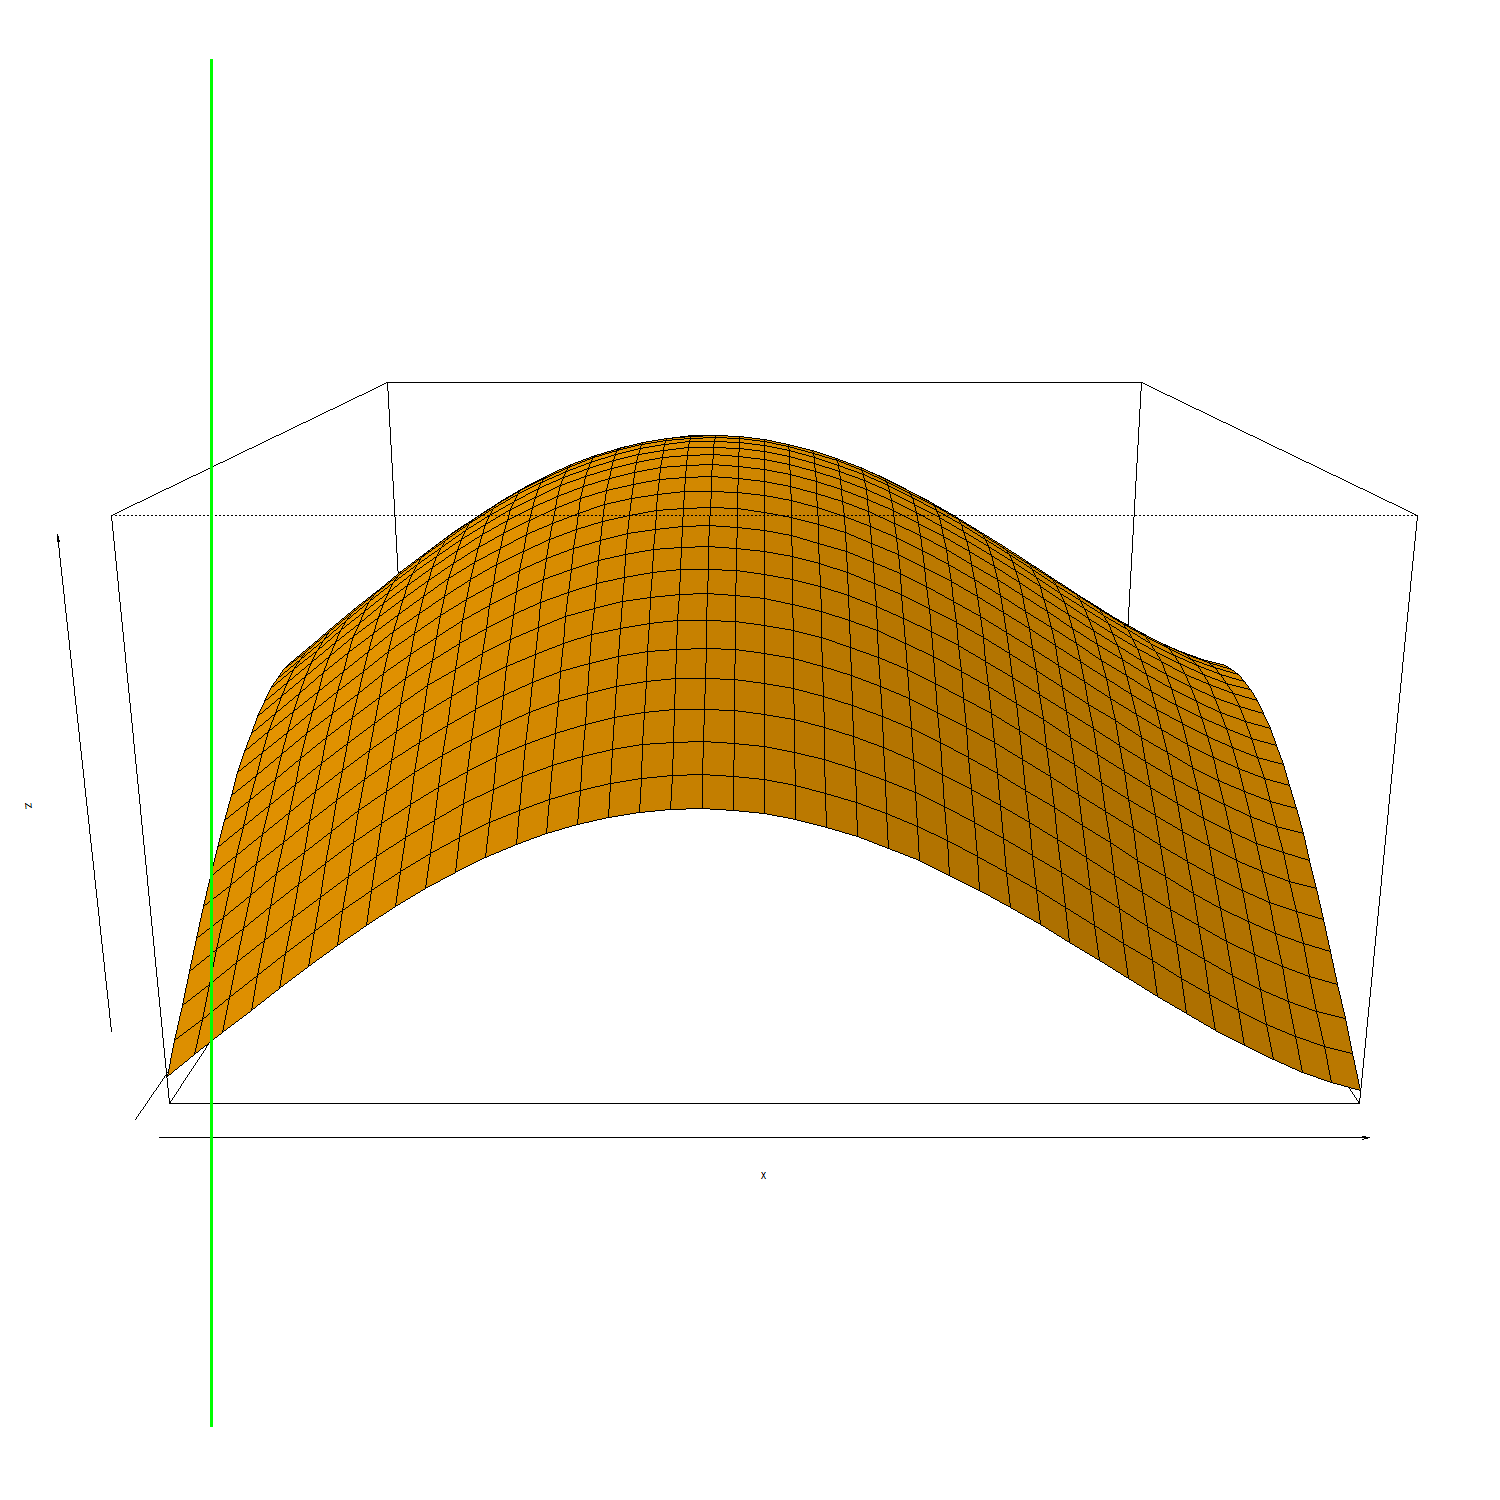
\includegraphics[width=7cm]{grafica_3D100.png}       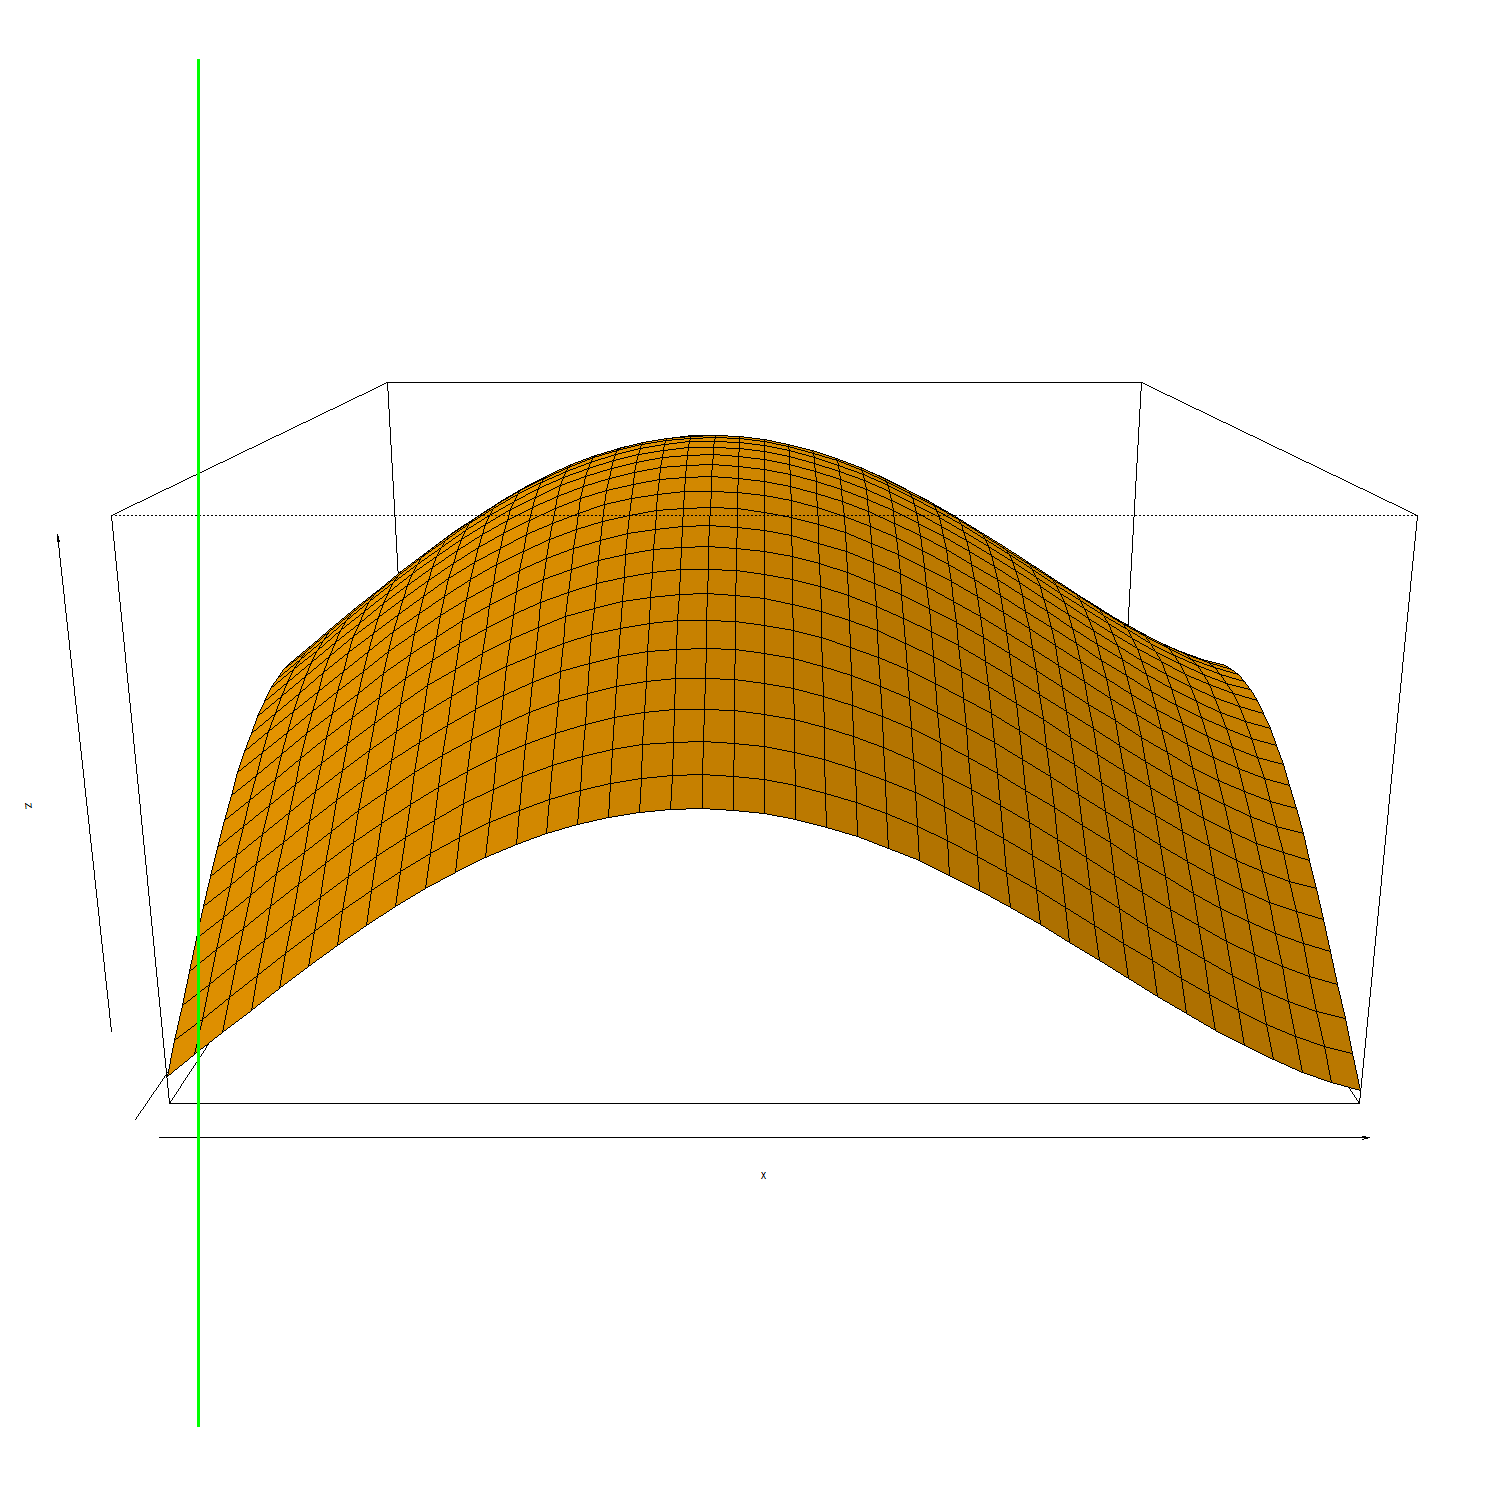
\includegraphics[width=7cm]{grafica_3D1000.png} 
\caption{Lado izquierda representa el análisis con 100 pasos y 1000 pasos el de la derecha}
\end{figure}

\begin{figure}[H]
\centering
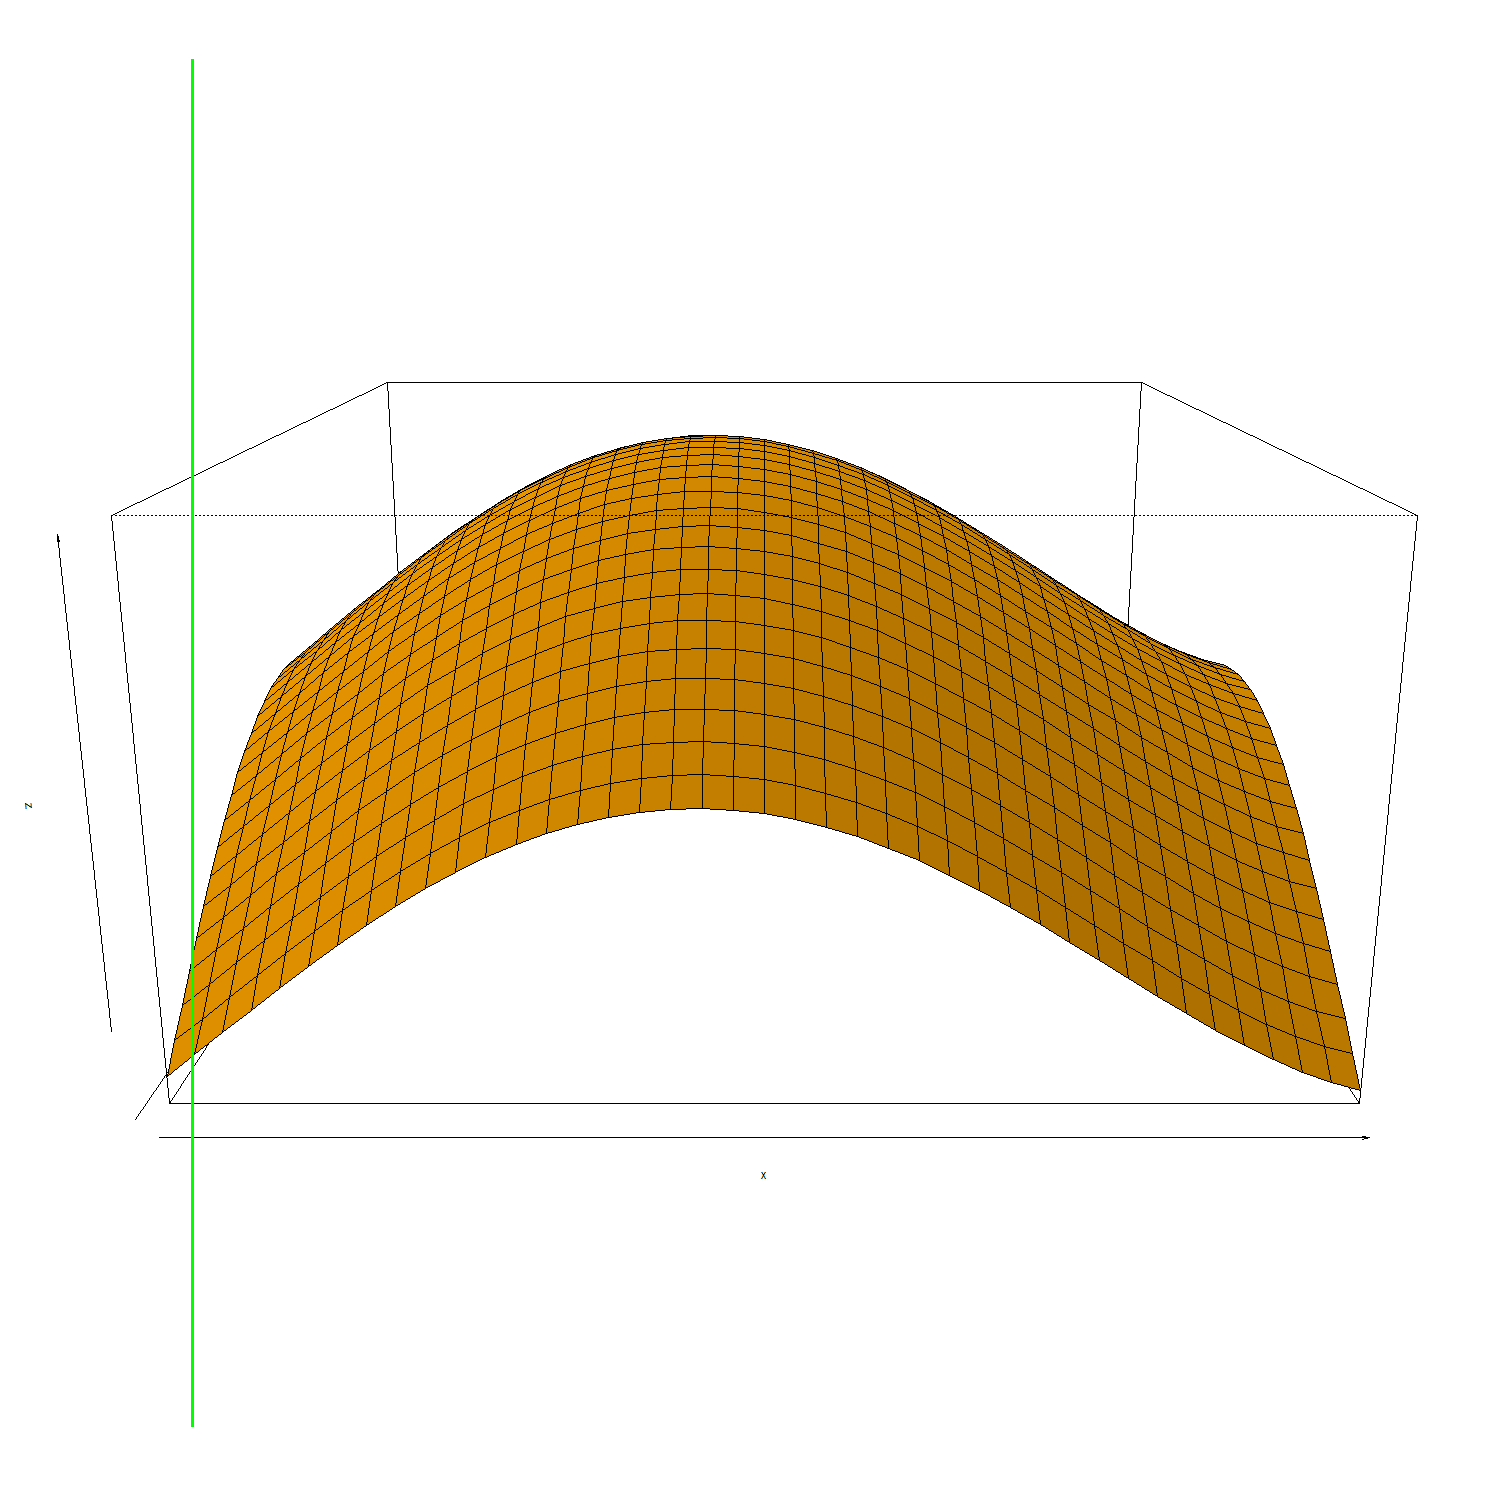
\includegraphics[width=7cm]{grafica_3D10000.png}
 \caption{Análsis de 10000 pasos}
\end{figure}

Las gráficas se obtuvieron con el siguiente código.
\begin{lstlisting}[frame=single]
suppressMessages(library(doParallel))
registerDoParallel(makeCluster(detectCores() - 1))

for (pot in 2:4) {
  tmax <- 10^pot
  resultados <- foreach(i = 1:replicas, .combine=c) %dopar% replica(tmax)
  png(paste("grafica_3D", tmax, ".png", sep=""), width=1500, height=1500)
  x <- seq(low, high, step)
  y <- x
  z <- outer(x, y, g)
  persp(x,y,z, col='orange',expand = 0.5, shade=0.2)
  valores <- f(resultados)
  points(resultados, valores, pch=1600, col="red")
  mejor <- which.max(valores)
  abline(v =resultados[mejor], col="green", lwd=3)
  graphics.off()
   }
stopImplicitCluster()

\end{lstlisting}


No se pudo realizar el mapa de calor (heatmap), el código es el siguiente:
\begin{lstlisting}[frame=single]
suppressMessages(library(doParallel))
registerDoParallel(makeCluster(detectCores() - 1))

for(graf in 2:4) {
  tmax <- graf
  resultados <- foreach(i = 1:replicas, .combine=c) %dopar% replica(tmax)
  valores <- f(resultados)
  mejor <- which.max(valores)
  x <- seq(low, high, step)
  y <- x
  z <- outer(x, y, g)
  dimnames(z) <- list(x, y)
  d <- melt(z)
  names(d) <- c("x", "y", "z")
  points(resultados, valores, pch=16, col="red")
  png("das.png", width=900, height=900)
  levelplot(z ~ x * y, data = d, main = "")
  graphics.off()
}

stopImplicitCluster()
\end{lstlisting}

\section{Conclusiones}
NA

\bibliographystyle{plainnat}
\bibliography{ref7}




\end{document}